\documentclass[12pt,a4paper,titlepage]{article}
\usepackage{License_style}
\usepackage{pdfpages}
\usepackage{eso-pic}

  
\begin{document}
\pagenumbering{gobble}


\numberwithin{lstlisting}{section}


% TITLE
\begin{titlepage}
\selectlanguage{romanian}

\newcommand{\HRule}{\rule{\linewidth}{0.5mm}} % Defines a new command for the horizontal lines, change thickness here

\center

Ministerul Educației al Republicii Moldova\\ % Name of your university/college
Universitatea Tehnică a Moldovei \\% Name of your university/college
Facultatea de Calculatoare, Informatică și Microelectronică\\
Filiera Anglofonă "Computer Science"\\


\vspace{2cm}
\vspace{2cm}



% \hfill Admis la susținere\\
% \hfill Șef de catedră: prof. dr. hab. Viorel Bostan\\

% \vspace{0.4cm}
% \hfill "\rule{0.75cm}{0.2mm}" \ \rule{3cm}{0.2mm} 2015
% \vspace{3cm}




\begin{center}
\Large \textbf{Stored procedures}\\
\vspace{0.6cm}
Proiect de an
\end{center}
\vspace{1cm}

\vspace{2cm}
\vspace{2cm}


\hfill Student: N.Botnari \\
\vspace{0.2cm}
\hfill A verificat: I. Cojanu



% If you don't want a supervisor, uncomment the two lines below and remove the section above
%\Large \emph{Author:}\\
%John \textsc{Smith}\\[3cm] % Your name

%----------------------------------------------------------------------------------------
%	DATE SECTION
%----------------------------------------------------------------------------------------
\vfill % Fill the rest of the page with whitespace
\begin{center}
Chișinău 2017
\end{center}


\end{titlepage}
\selectlanguage{english}


\cleardoublepage


\tableofcontents

\newpage

\pagenumbering{arabic}
\setcounter{page}{10}
\setcounter{secnumdepth}{4}

\addtocontents{toc}{\protect\thispagestyle{empty}} % no page number on the table of contents page
\cleardoublepage


%LISTA FIGURILOR. Este recomandabila daca in text ai peste cel putin 10-15 FIGURI
% \listoffigures
% \addcontentsline{toc}{section}{List of figures}
% \clearpage

%LISTA TABELELOR. Este recomandabila daca in text ai peste cel putin 10-15 tabele
% \listoftables
% \addcontentsline{toc}{section}{List of tables}
% \clearpage

\lstlistoflistings
\addcontentsline{toc}{section}{Listings}
\clearpage

%INTRODUCERE
%\setcounter{page}{17} 
\phantomsection
\addcontentsline{toc}{section}{Introduction}
\section*{Introduction to Stored procedures}
\phantomsection

Stored procedures have been viewed as the de facto standard for applications to access and manipulate database information through the use of codified methods, or “procedures.” This is largely due to what they offer developers: the opportunity to couple the set-based power of SQL with the iterative and conditional processing control of code development. Developers couldn’t be happier about this; finally, instead of writing inline SQL and then attempting to manipulate the data from within the code, developers could take advantage of:\\
\textbf{Familiar Coding Principles}
\begin{enumerate}
\item Iterative Loops
\item Conditionals
\item Method Calls (the stored procedure itself is built and similarly called like a method)
\end{enumerate}
\textbf{One-time, One-place Processing}
\begin{enumerate}
\item Instead of having inline SQL code spread throughout the application, now sections of SQL code can be encapsulated into chunks of named methods that are easily identifiable and accessible all within one location – the “Stored Procedure” folder of the database.
\item All complex data processing can now be performed on the server, allowing the client processing to focus more on presentation rather than manipulation of data.
\end{enumerate}

Of course, just because something is popular doesn’t always mean that it’s the best tool in all situations. The efficiency, efficacy and utility of Stored Procedures, just like the implementation of all programming languages and platforms, are all dependent on the needs of the client and the subsequent architecture of the application.



\clearpage
\cleardoublepage

% CAPITOLUL 1
\section{SQL Stored procedures}
\phantomsection

A stored procedure in SQL Server is a group of one or more Transact-SQL statements or a reference to a Microsoft .NET Framework common runtime language (CLR) method. Procedures resemble constructs in other programming languages because they can:
\begin{itemize}
  \item[$\bullet$] Accept input parameters and return multiple values in the form of output parameters to the calling program.
  \item[$\bullet$] Contain programming statements that perform operations in the database. These include calling other procedures.
  \item[$\bullet$] Return a status value to a calling program to indicate success or failure (and the reason for failure).
\end{itemize}
\subsection{Types of Stored Procedures}
There are several types of Stored procedures in SQL Server: \\
\textbf{User-defined}\\
A user-defined procedure can be created in a user-defined database or in all system databases except the Resource database. The procedure can be developed in either Transact-SQL or as a reference to a Microsoft .NET Framework common runtime language (CLR) method.\\
\textbf{Temporary}\\
Temporary procedures are a form of user-defined procedures. The temporary procedures are like a permanent procedure, except temporary procedures are stored in tempdb. There are two types of temporary procedures: local and global. They differ from each other in their names, their visibility, and their availability. Local temporary procedures have a single number sign (\#) as the first character of their names; they are visible only to the current user connection, and they are deleted when the connection is closed. Global temporary procedures have two number signs  as the first two characters of their names; they are visible to any user after they are created, and they are deleted at the end of the last session using the procedure.\\
\textbf{System}\\
System procedures are included with SQL Server. They are physically stored in the internal, hidden Resource database and logically appear in the sys schema of every system- and user-defined database. In addition, the msdb database also contains system stored procedures in the dbo schema that are used for scheduling alerts and jobs.\\
\textbf{Extended User-Defined}\\
Extended procedures enable creating external routines in a programming language such as C. These procedures are DLLs that an instance of SQL Server can dynamically load and run.

\subsection{Benefits of Using the Stored Procedure}

\begin{enumerate}
\item One of the main benefits of using the Stored procedure is that it reduces the amount of information sent to the database server. It can become a more important benefit when the bandwidth of the network is less. Since if we send the SQL query (statement) which is executing in a loop to the server through network and the network gets disconnected, then the execution of the SQL statement doesn't return the expected results, if the SQL query is not used between Transaction statement and rollback statement is not used.
\item Compilation step is required only once when the stored procedure is created. Then after it does not require recompilation before executing unless it is modified and reutilizes the same execution plan whereas the SQL statements need to be compiled every time whenever it is sent for execution even if we send the same SQL statement every time.
\item It helps in re usability of the SQL code because it can be used by multiple users and by multiple clients since we need to just call the stored procedure instead of writing the same SQL statement every time. It helps in reducing the development time.
\item Stored procedure is helpful in enhancing the security since we can grant permission to the user for executing the Stored procedure instead of giving permission on the tables used in the Stored procedure.
\item Sometimes, it is useful to use the database for storing the business logic in the form of stored procedure since it makes it secure and if any change is needed in the business logic, then we may only need to make changes in the stored procedure and not in the files contained on the web server.
\end{enumerate}

\subsection{How to Create a Stored Procedure in SQL Server}
We need to give the procedure a unique name within the schema and then write the sequence of SQL statements to be executed within the procedure. Following is the basic syntax for creating stored procedures:
\lstinputlisting[style=mystyle, language=SQL, caption={Template of a procedure, \cite{doc}}, label=list41,]{sourcecode/tsqlexample.sql}

This template contains parameters for parameter names, procedure name, author name, create date, and so on. These template parameters are in the format <parameter, type, value>:
PARAMETER\_NAME: It is the name of the template parameter in the script.
DATA\_TYPE: It is the optional data type of the template parameter.
VALUE: It is the default value to be used to replace every occurrence of the template parameter in the script.
SET NOCOUNT ON:

1) It gives performance. When SET NOCOUNT is ON, the count (indicating the number of rows affected by a Transact-SQL statement) is not returned. 
2) When SET NOCOUNT is OFF, the count is returned. It eliminates the sending of ONE\_IN\_PROC messages to the client for each statement in a stored procedure. 
3) For stored procedures that contain several statements that do not return much actual data, this can provide a significant performance boost because network traffic is greatly reduced. The setting of SET NOCOUNT is set at execute or run time and not at parse time.
 
RETURN:

1) Return values indicate a return code from the stored procedure. The return value does not have to be specified as the parameters do. We simply use the RETURN SQL statement to return a value. This value has to be an Integer data type and can return any value you need. For example, this value can be a return code, the number of rows affected by a SQL statement, or the number of rows in a table. Basically any integer data that you want to return can be specified in a return value in your stored procedure.

2) The RETURN statement exits unconditionally from a stored procedure, so the statements following RETURN are not executed. Though the RETURN statement is generally used for error checking, you can use this statement to return an integer value for any other reason. Using RETURN statement can boost performance because SQL Server will not create a recordset.

% \lstinputlisting[style=mystyle, language=SQL, caption={Caption of the listing code, \cite{doc}}, label=list41,]{sourcecode/minmax.sql}

% \begin{figure}[ht!]
%     \centering
%     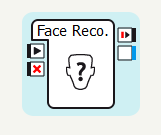
\includegraphics[width=0.2\textwidth]{face_reco}
%     \caption{}
%     \label{fig_21}
% \end{figure}

\clearpage
\cleardoublepage
%
%CAPITOLUL2
\section{Oracle SQL Stored Procedures (Subprograms)}
\phantomsection
\subsection{About Subprograms}
Subprograms are named PL/SQL blocks that can take parameters and be invoked. PL/SQL has two types of subprograms called procedures and functions. Generally, you use a procedure to perform an action and a function to compute a value.

Like unnamed or anonymous PL/SQL blocks, subprograms have a declarative part, an executable part, and an optional exception-handling part. The declarative part contains declarations of types, cursors, constants, variables, exceptions, and nested subprograms. These items are local and cease to exist when you exit the subprogram. The executable part contains statements that assign values, control execution, and manipulate Oracle data. The exception-handling part contains exception handlers, which deal with exceptions raised during execution.

Consider the following procedure named debit\_account, which debits a bank account:

\lstinputlisting[style=mystyle, language=SQL, caption={Example of subprogram, \cite{doc}}, label=list41,]{sourcecode/debit.sql}

When invoked or called, this procedure accepts an account number and a debit amount. It uses the account number to select the account balance from the accts database table. Then, it uses the debit amount to compute a new balance. If the new balance is less than zero, an exception is raised; otherwise, the bank account is updated.

\subsection{Advantages of Subprograms}
Subprograms provide extensibility; that is, they let you tailor the PL/SQL language to suit your needs.Subprograms also provide modularity; that is, they let you break a program down into manageable, well-defined logic modules. This supports top-down design and the stepwise refinement approach to problem solving.

Also, subprograms promote reusability and maintainability. Once validated, a subprogram can be used with confidence in any number of applications. Furthermore, only the subprogram is affected if its definition changes. This simplifies maintenance and enhancement.

Finally, subprograms aid abstraction, the mental separation from particulars. To use subprograms, you must know what they do, not how they work. Therefore, you can design applications from the top down without worrying about implementation details. Dummy subprograms (stubs) allow you to defer the definition of procedures and functions until you test and debug the main program.

\subsection{Procedures}
A procedure is a subprogram that performs a specific action. You write procedures using the syntax
\lstinputlisting[style=mystyle, language=SQL, caption={Example of a procedure in SQL Oracle, \cite{doc}}, label=list41,]{sourcecode/prodexample.sql}
where parameter stands for the following syntax:

parameter\_name [IN | OUT | IN OUT] datatype [{:= | DEFAULT} expression]

You cannot impose the NOT NULL constraint on a parameter.

Also, you cannot specify a constraint on the datatype. For example, the following declaration of emp\_id is illegal because it imposes a size constraint:

PROCEDURE raise\_salary (emp\_id NUMBER(4)) IS ...  -- illegal; should be NUMBER

A procedure has two parts: the specification and the body. The procedure specification begins with the keyword PROCEDURE and ends with the procedure name or a parameter list. Parameter declarations are optional. Procedures that take no parameters are written without parentheses.

The procedure body begins with the keyword IS and ends with the keyword END followed by an optional procedure name. The procedure body has three parts: a declarative part, an executable part, and an optional exception-handling part.

The declarative part contains local declarations, which are placed between the keywords IS and BEGIN. The keyword DECLARE, which introduces declarations in an anonymous PL/SQL block, is not used. The executable part contains statements, which are placed between the keywords BEGIN and EXCEPTION (or END). At least one statement must appear in the executable part of a procedure. The NULL statement meets this requirement. The exception-handling part contains exception handlers, which are placed between the keywords EXCEPTION and END.

Consider the procedure raise\_salary, which increases the salary of an employee:
\lstinputlisting[style=mystyle, language=SQL, caption={Procedure in SQL Oracle, \cite{doc}}, label=list41,]{sourcecode/salary.sql}
When called, this procedure accepts an employee number and a salary increase amount. It uses the employee number to select the current salary from the emp database table. If the employee number is not found or if the current salary is null, an exception is raised. Otherwise, the salary is updated.

A procedure is called as a PL/SQL statement. For example, you might call the procedure raise\_salary as follows:

raise\_salary(emp\_num, amount);

\subsection{Stored Subprograms}
Generally, tools (such as Oracle Forms) that incorporate the PL/SQL engine can store subprograms locally for later, strictly local execution. However, to become available for general use by all tools, subprograms must be stored in an Oracle database.

To create subprograms and store them permanently in an Oracle database, you use the CREATE PROCEDURE and CREATE FUNCTION statements, which you can execute interactively from SQL*Plus or Enterprise Manager. For example, you might create the procedure fire\_employee, as follows:

\lstinputlisting[style=mystyle, language=SQL, caption={Stored subprograms in SQL Oracle, \cite{doc}}, label=list41,]{sourcecode/storedproc.sql}

When creating subprograms, you can use the keyword AS instead of IS in the specification for readability.


\clearpage
\cleardoublepage

%CAPITOLUL3
\section{Comparision between Stored procedures in PL-SQL and T-SQL}
\phantomsection

\subsection{Overloading}
\textbf{Overloading is present only in SQL Oracle and is not supported by Sql Server.}\\

PL/SQL lets you overload subprogram names. That is, you can use the same name for several different subprograms as long as their formal parameters differ in number, order, or datatype family.\\

Suppose you want to initialize the first n rows in two index-by tables that were declared as follows:

\lstinputlisting[style=mystyle, language=SQL, caption={Tables, \cite{doc}}, label=list41,]{sourcecode/table.sql}

You might write the following procedure to initialize the index-by table named hiredate\_tab:

\lstinputlisting[style=mystyle, language=SQL, caption={First procedure, \cite{doc}}, label=list41,]{sourcecode/init1.sql}

And, you might write the next procedure to initialize the index-by table named sal\_tab:

\lstinputlisting[style=mystyle, language=SQL, caption={First procedure, \cite{doc}}, label=list41,]{sourcecode/init2.sql}

Because the processing in these two procedures is the same, it is logical to give them the same name.

You can place the two overloaded initialize procedures in the same block, subprogram, or package. PL/SQL determines which of the two procedures is being called by checking their formal parameters.

Consider the example below. If you call initialize with a DateTabTyp parameter, PL/SQL uses the first version of initialize. But, if you call initialize with a RealTabTyp parameter, PL/SQL uses the second version.
\lstinputlisting[style=mystyle, language=SQL, caption={Calling both procedures, \cite{doc}}, label=list41,]{sourcecode/inittable.sql}

\subsection{Packages}
\textbf{Packages are present only in SQL Oracle and are not supported by Sql Server.}\\

The specification is the interface to the package. It just DECLARES the types, variables, constants, exceptions, cursors, and subprograms that can be referenced from outside the package. In other words, it contains all information about the content of the package, but excludes the code for the subprograms.

All objects placed in the specification are called public objects. Any subprogram not in the package specification but coded in the package body is called a private object.

The following code snippet shows a package specification having a single procedure. You can have many global variables defined and multiple procedures or functions inside a package.
\lstinputlisting[style=mystyle, language=SQL, caption={Package, \cite{doc}}, label=list41,]{sourcecode/package.sql}

%\begin{figure}[h]
%    \centering
%    \includegraphics[width=0.80\textwidth]{nao_monitor}
%    \caption{ Monitor Desktop}
%    \label{fig:mesh7}
%\end{figure}


\clearpage
\cleardoublepage


% IMPORTANT REMARK  
% If your table of contents need to be splitted in two parts (in order to accomodate the frame used for TOC)
% within the body text, right before the chapter/section that you want to be started on anew page, 
% you should add:     \addtocontents{toc}{\protect\newpage}

%CONCLUZII
\phantomsection
\addcontentsline{toc}{section}{Conclusions}
\section*{Conclusions}
\phantomsection

In this project, I covered the fundamentals of stored procedures and some specific properties pertaining to them. Of course, I should continue your studies in areas like security, SQL statements, and performance before you can master SQL routines.\par
Stored Procedures may not always be the right answer for processing data, but there’s also not enough compelling evidence to not use them either. Whether or not to use them determines on your particular situation and ability to develop the Stored Procedure(s) to match. Just like with writing a good, quality application, if you or your developers can write good, quality Stored Procedures, then by all means implement them. If they can’t, then another solution might be best for you.\par
I generally use procedures, their benefits in terms of security, code maintenance and software design make them worthy of use, in my opinion.

\clearpage
\cleardoublepage

\cleardoublepage
\addcontentsline{toc}{section}{References}
\begin{thebibliography}{99999}
\phantomsection
\singlespace\normalsize

\bibitem{SQLServerOfficial} SQL Server Documentation, \textit{ official page}, \url{https://docs.microsoft.com/en-us/sql/sql-server/sql-server-technical-documentation}

\bibitem{SQLOracleOfficial} SQL Oracle Documentation, \textit{ official page}, \url{https://docs.oracle.com/cd/B19306_01/server.102/b14200/toc.htm}

\bibitem{seguetech} Seguetech, \textit{ official page}, \url{http://www.seguetech.com/advantages-and-drawbacks-of-using-stored-procedures-for-processing-data/}

\end{thebibliography}

\cleardoublepage
   
 
\end{document}